\documentclass[12pt,a4paper]{report} %How the pages are set up
\usepackage[british,UKenglish,USenglish,english,american]{babel} %set which langue the name of things are
\usepackage{fancyhdr} %package to change the headder and fotter
\usepackage{lastpage} %package to be able to reference the pagenumber of the last page
\usepackage{tocloft} %package to change the formating of the table of contents
\usepackage{hyperref} %package to put links in the pdf (and make the table of contents lines to links to the respective lines)
\usepackage{xcolor}
\usepackage{color} %package to have a static reference to colors
\usepackage{titlesec} %package to change the formatting of the titles
\usepackage{datetime} %package to reference the current date and time
\usepackage[pdftex]{graphicx} %package to set default layout when compiling
\usepackage[utf8]{inputenc} %package to set the typeset
\usepackage{gensymb} %package to add some mathematical symbols
\usepackage{cite} %package to be able to quote stuff
\usepackage{enumitem} %package to change formatting of lists
\usepackage{rotating} %package to be able to rotate figures
\usepackage{caption}%package to add captions to pictures
\usepackage{longtable}%package to make tables that span multiple pages
\usepackage{listings}
\usepackage{hyperref}
\usepackage{atbegshi}
\usepackage{pdfpages}
%\renewcommand\bibname{Kildehenvisning}


\AtBeginDocument{\AtBeginShipoutNext{\AtBeginShipoutDiscard{}}}
\addto\captionsdanish{
  \renewcommand{\bibname}
    {Kildehenvisning}
}

\addto\captionsdanish{
  \renewcommand{\contentsname}
    {Indholdsfortegnelse}}

%\hypersetup{colorlinks,urlcolor=blue}
\addtocontents{toc}{\protect\thispagestyle{empty}}
\setlength{\parindent}{2em}
\linespread{1.2}
\setlist[itemize]{itemsep=0mm}
\definecolor{gray75}{gray}{0.75}
\newcommand{\hsp}{\hspace{20pt}}
\newcommand{\bhref}[2]{\color{blue}{\href{#1}{#2}}\color{black}}
\titleformat{\chapter}[hang]{\Huge\bfseries}{\thechapter\hsp\textcolor{gray75}{$|$}\hsp}{0pt}{\Huge\bfseries}
\titlespacing*{\chapter}{0pt}{-50pt}{40pt}
\setlength{\parskip}{1em}
%\renewcommand{\headsep}{-3em}

\title{
    \vspace{2em}\newline 
    Compilerteknik
}
\author{
\resizebox{\columnwidth}{!}{
\begin{tabular}{ccc}
Rasmus T. N.,                             &                    & Michael J.,                           \\
s185101                                  &                        & s185123                               \\

\includegraphics[width=29mm,height=106,scale=0.2]{Billeder/Personer/RasmusTarubNielsen1.jpg}&
\includegraphics[]{Billeder/Personer/white.PNG}&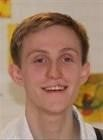
\includegraphics[]{Billeder/Personer/MichaelJeppesen.jpg}\\
\newline
Nicklas C. F.,                           &               & Philip B. Ø.,                          \\
s180087                                  &               &s185137                                \\
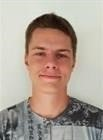
\includegraphics[]{Billeder/Personer/NicklasChristofferFritzen.jpg}&&
\includegraphics[]{Billeder/Personer/PhilipBocayesOernskov.jpg} 
\end{tabular}}
}
\date{\vspace{-1em}\hspace{4em}\today\newline
\url{https://github.com/Fipzz/Compilerteknik-Assingment-1}
}
\newpage
\pagestyle{fancyplain}
\fancyhf{}
\fancyhead{}
\fancyfoot{}
\fancyhead[C]{Assignment 1}
\fancyhead[L]{}
\fancyhead[R]{\today}
\fancyfoot[C]{Side \thepage\ af \pageref{LastPage}}
\fancyfoot[R]{}

\fancypagestyle{firstpage}{%
  
  \rhead{}
  \fancyfoot{}
}

\begin{document}
   
    \begin{titlepage}
    %\centering
    \pagestyle{firstpage}
    \maketitle
%    \thispagestyle{empty}
    \end{titlepage}
    \pagestyle{fancyplain}

    \section*{Task 1}

    Inde i .g4 filen har vi ændret på grammatikken, så den ser således ud:
    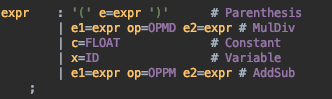
\includegraphics[scale=0.7]{Billeder/Bilag/expressions.png}\\
    Det har vi gjort, for at slå Multiplication+Division sammen og Addition+Subtraction sammen. Det gør vi for at spare metoder og sikre at det matematiske hierarki bliver overholdt og der ikke sker forkerte udregninger.
    
    Dette medfører at vores metoder i .java filen ser således ud:\\
    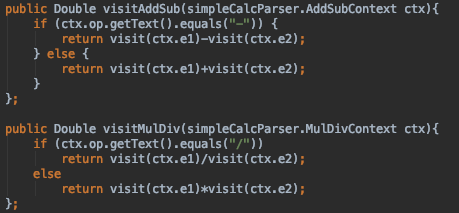
\includegraphics[scale=0.7]{Billeder/Bilag/methods.png}\\
    Siden vi har kombineret, håndterer vores metoder inputtet og bestemmer om den skal gange/dividere eller plusse/minuse. Dette sikre også at det bliver korrekt udregnet.


    \section*{Task 2}
    
    Vi har valgt at design vores grammatik og syntax, så det ligner java's syntax. Vi føler os komfortable med java's syntax og vi ved hvordan vi skal designe grammatik efter det. Vi følte det unødvendigt at designe at sprog lignende LOLCODE eller lignende.
    
    \section*{Task 3}
    Vi har udvidet vores .g4 fil, så det nu ligner et programeringssporg. Dette har vi gjordt ved at tilføje funktioner som "While", "If", "Else if", "Else" og bitwise operatorer. 
    We have also devoloped small test for our new 
    

    
    \subsection*{Tests}
    
    \section*{Task 4}
    De fleste af de grammatiske regler vi har implementeret er basale og er bare varianter af denne:
    
    
\end{document}
